\documentclass[11pt,notheorems,hyperref={pdfauthor=whatever}]{beamer}


% Copyright (c) 2022 by Lars Spreng
% This work is licensed under the Creative Commons Attribution 4.0 International License. 
% To view a copy of this license, visit http://creativecommons.org/licenses/by/4.0/ or send a letter to Creative Commons, PO Box 1866, Mountain View, CA 94042, USA.

%~~~~~~~~~~~~~~~~~~~~~~~~~~~~~~~~~~~~~~~~~~~~~~~~~~~~~~~~~~~~~~~~~~~~~~~~~~~~~~
% Add your packages and commands to this file
%~~~~~~~~~~~~~~~~~~~~~~~~~~~~~~~~~~~~~~~~~~~~~~~~~~~~~~~~~~~~~~~~~~~~~~~~~~~~~~

%~~~~~~~~~~~~~~~~~~~~~~~~~~~~~~~~~~~~~~~~~~~~~~~~~~~~~~~~~~~~~~~~~~~~~~~~~~~~~~
\RequirePackage{palatino}
\RequirePackage[utf8]{inputenc}
\RequirePackage[T1]{fontenc}

\usefonttheme{serif}

\usepackage{styles/elegantmacros}
\usefolder{styles}
\usetheme[style=blue]{elegant}

\newcommand{\makepart}[1]{ % For convenience
\part{#1} \frame{\partpage}
}

%~~~~~~~~~~~~~~~~~~~~~~~~~~~~~~~~~~~~~~~~~~~~~~~~~~~~~~~~~~~~~~~~~~~~~~~~~~~~~~

%~~~~~~~~~~~~~~~~~~~~~~~~~~~~~~~~~~~~~~~~~~~~~~~~~~~~~~~~~~~~~~~~~~~~~~~~~~~~~~
% Figures
\RequirePackage{booktabs}
\RequirePackage{colortbl}
\RequirePackage{ragged2e}
\RequirePackage{schemabloc}
%\RequirePackage{natbib}
\RequirePackage{caption}
\RequirePackage{subcaption}
\RequirePackage{tabularx}
\RequirePackage{array}
\RequirePackage{multirow}
\usepackage[
  style=authoryear, 
]{biblatex}
\addbibresource{references.bib}
\newcolumntype{Y}{>{\centering\arraybackslash}X}

%~~~~~~~~~~~~~~~~~~~~~~~~~~~~~~~~~~~~~~~~~~~~~~~~~~~~~~~~~~~~~~~~~~~~~~~~~~~~~~

%~~~~~~~~~~~~~~~~~~~~~~~~~~~~~~~~~~~~~~~~~~~~~~~~~~~~~~~~~~~~~~~~~~~~~~~~~~~~~~
% Figures
\RequirePackage{wrapfig}
\RequirePackage{pgfplots}
\RequirePackage{graphicx}
\RequirePackage{adjustbox}
\RequirePackage{environ}
\pgfplotsset{compat=1.18}

\makeatletter
\newsavebox{\measure@tikzpicture}
\NewEnviron{scaletikzpicturetowidth}[1]{%
  \def\tikz@width{#1}%
  \def\tikzscale{1}\begin{lrbox}{\measure@tikzpicture}%
  \BODY
  \end{lrbox}%
  \pgfmathparse{#1/\wd\measure@tikzpicture}%
  \edef\tikzscale{\pgfmathresult}%
  \BODY
}
\makeatother
%~~~~~~~~~~~~~~~~~~~~~~~~~~~~~~~~~~~~~~~~~~~~~~~~~~~~~~~~~~~~~~~~~~~~~~~~~~~~~~

%~~~~~~~~~~~~~~~~~~~~~~~~~~~~~~~~~~~~~~~~~~~~~~~~~~~~~~~~~~~~~~~~~~~~~~~~~~~~~~
% Maths 
\RequirePackage{textcomp}
\RequirePackage{amsmath} 
\RequirePackage{amsthm}
\RequirePackage{mathtools}
%\RequirePackage{bbm}
%\RequirePackage{algorithm}
%\RequirePackage[osf,sc]{mathpazo}
%\RequirePackage{pifont}
%\newcommand{\xmark}{\ding{55}}%
%\numberwithin{equation}{section}
\DeclareMathOperator*{\argmax}{arg\,max}
\DeclareMathOperator*{\argmin}{arg\,min}

\setbeamertemplate{theorems}[numbered] % to number

\theoremstyle{definition}
\newtheorem{fact}{Fact}[section]
\newtheorem{examp}{Example}[section]

\theoremstyle{plain}
\newtheorem{definition}{Definition}[section]
\newtheorem{proposition}{Proposition}
\newtheorem{theorem}{Theorem}
\newtheorem{assumption}{Assumption}
\setbeamertemplate{caption}[numbered]

\providecommand{\H}{\mathscr{H}}      
\providecommand{\E}{\mathbb{E}}
\makeatletter
\def\munderbar#1{\underline{\sbox\tw@{$#1$}\dp\tw@\z@\box\tw@}}
\makeatother

%~~~~~~~~~~~~~~~~~~~~~~~~~~~~~~~~~~~~~~~~~~~~~~~~~~~~~~~~~~~~~~~~~~~~~~~~~~~~~~
 % Loads packages and some defined commands


\title[]{Generalisation, Inductive Learning, Structured Data and When to Use ML?}

\author[]{Sagar Prakash Barad \& Sajag Kumar}

\institute{
    National Institute of Science Education and Research (NISER) \\ 
    Bhubaneswar}
\date{\today}

\begin{document}

{
\setbeamertemplate{footline}{} 
\begin{frame}
  \titlepage
\end{frame}
}
\addtocounter{framenumber}{-1}

\begin{frame}{Part I: Some Terminology}
    \tableofcontents[part=1]
\end{frame}
\begin{frame}{Part II: Generalization and Inductive Learning}
    \tableofcontents[part=2]
\end{frame}
\begin{frame}{Part III: Structured Data and When to Use Machine Learning}
    \tableofcontents[part=3]
\end{frame}

\makepart{Some Terminology}

\section{Artificial Intelligence}
\begin{frame}{Artificial Intelligence}
The \alert{\textbf{Oxford Dictionary of English}} defines intelligence as 'the ability to acquire and apply knowledge and skills.`
\begin{itemize}
    \item Notice that to be called intelligent one should just be able to acquire some knowledge or skill and apply it. But in common usage, we refer to someone as intelligent when they are able to acquire and apply the knowledge and skills well.
    \item \alert{\textbf{Artificial intelligence}} is the ability of machines to acquire and apply knowledge and skills.
    \item To quantify the intelligence of machines, the standard convention is to compare it with humans. We call a machine intelligent, if it is as good as humans at a certain task. If a machine is better than humans in all tasks, we call it \alert{\textbf{superintelligent}} (such a machine does not exist).
\end{itemize}
\end{frame}

\begin{frame}{Examples of Artificial Intelligence}
\begin{enumerate}
    \item \alert{AlphaZero}, the famous chess-playing engine developed by DeepMind. It can defeat any human or other chess-playing engine quite easily, hence it is intelligent. However, it is not superintelligent despite being better than humans at chess because it cannot outperform humans in other tasks, for example, speech recognition.
    \item \alert{Alexa}, is a virtual assistant developed by Amazon. It recognises verbal instructions and, based on them, performs certain tasks. Alexa is as good as humans in speech recognition and hence is intelligent. But again not superintelligent because it cannot, for example, play chess.
\end{enumerate}
\end{frame}

\section{Deterministic and Non-Deterministic Algorithms}
\begin{frame}{Deterministic and Non-Deterministic Algorithms}
In machine learning we will come across a number of algorithms. All of these algorithms can be broadly classified into two categories:
\begin{enumerate}
    \item \alert{\textbf{Deterministic Algorithms}}: Given an input, output is always the same, and the machine on which the algorithm is running when given same input produces the output in exactly the same way.
    \item \alert{\textbf{Non-Deterministic Algorithms}}: Given an input, the machine on which the algorithm is running produces the output in different ways, the output may or may not be the same for same input. 
\end{enumerate}
\end{frame}

\begin{frame}[allowframebreaks]{Examples}
\bigskip
\begin{enumerate}
    \item \alert{\textbf{Deterministic Finite Automaton (DFA)}}: The following DFA is an example of a deterministic machine. Given same input the machine goes through exactly the same states every time to produce the same output.
    \bigskip
    \begin{figure}
    \centering
    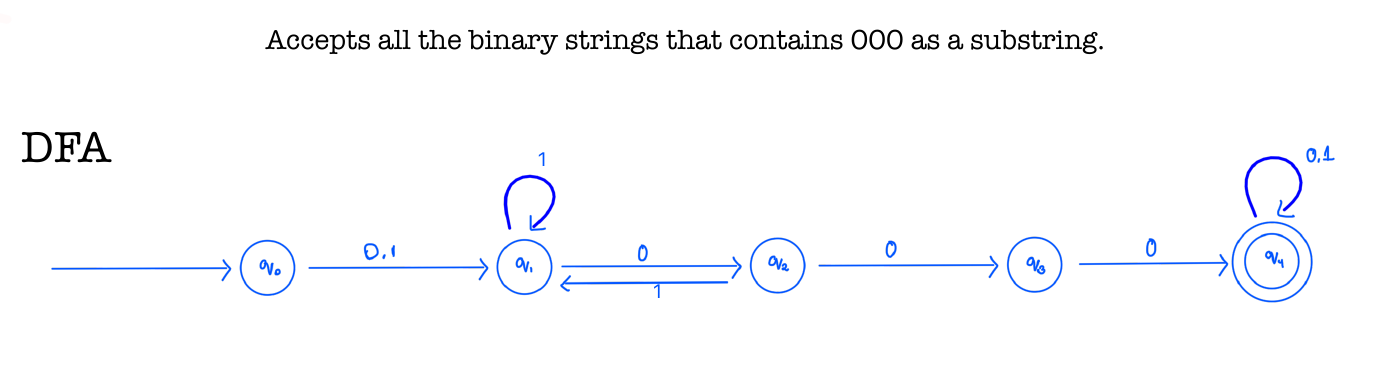
\includegraphics[width=0.9\textwidth]{figures/exp1_1.png}
    \caption{At state $q_1$ for input '0' and '1', one can determine the state to which machine will move.}
    \label{fig:DFA}
    \end{figure}
    \bigskip
    \item \alert{\textbf{Non-Deterministic Finite Automaton (NFA)}}: The following NFA is an example of a non-deterministic machine. Given same input the machine produces the same output but it can go through different set of states.
    \bigskip
    \begin{figure}
    \centering
    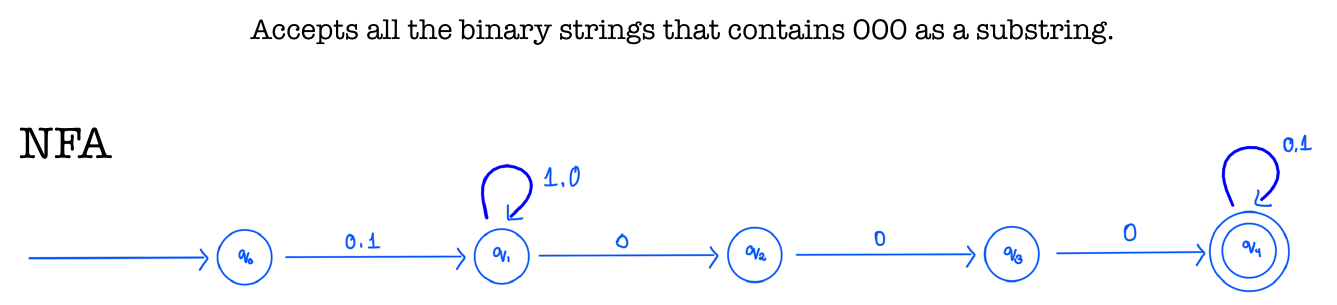
\includegraphics[width=0.9\textwidth]{figures/exp1_2.png}
    \caption{At state $q_1$ for input '0' machine can move to either state $q_1$ or $q_0$. Thus the exact state to which the machine will move cannot be determined.}
    \label{fig:NFA}
    \end{figure}
\end{enumerate}
\end{frame}

\makepart{Generalization}

\section{Learning}
\begin{frame}[allowframebreaks]{What is learning?}
\begin{itemize}
    \item Consider a \alert{teacher T}, \alert{student S} and a \alert{subject S1}. The teacher T, wants to know if the student S, learned the subject S1.
    \item \alert{T} in order to teach \alert{S1} provides some \alert{notes} to \alert{S}.
    \item \alert{T} wants to know if \alert{S} learned from the notes.
    \item A parameter for learning would be how good \alert{S} does on an exam.
    \item \alert{T} can take three kinds of exam to judge if \alert{S} actually learned \alert{S1}:
    \begin{enumerate}
        \item Put all the questions directly from the notes.
        \item Put questions from a subject other than \alert{S1}.
        \item Put questions based on the notes but not directly from them. 
    \end{enumerate}
    \bigskip
    \item Lets see which of these exams can tell us if \alert{S} learned \alert{S1} based on their performance.
    \begin{enumerate}
        \item If \alert{S} does well on the first exam it would mean that they are good at memorising. They memorised everything from the notes and reproduced on the exam. 
        \item If \alert{S} does well on the second exam. Either they are extremely lucky or they are God. This type of an exam is not a good way of gauging whether \alert{S} actually learned anything.
        \item If \alert{S} does well on the third exam it would imply they have learned from the notes. Because they could answer questions based on what they learned from the notes. 
    \end{enumerate}
\end{itemize}
\begin{figure}
    \centering
    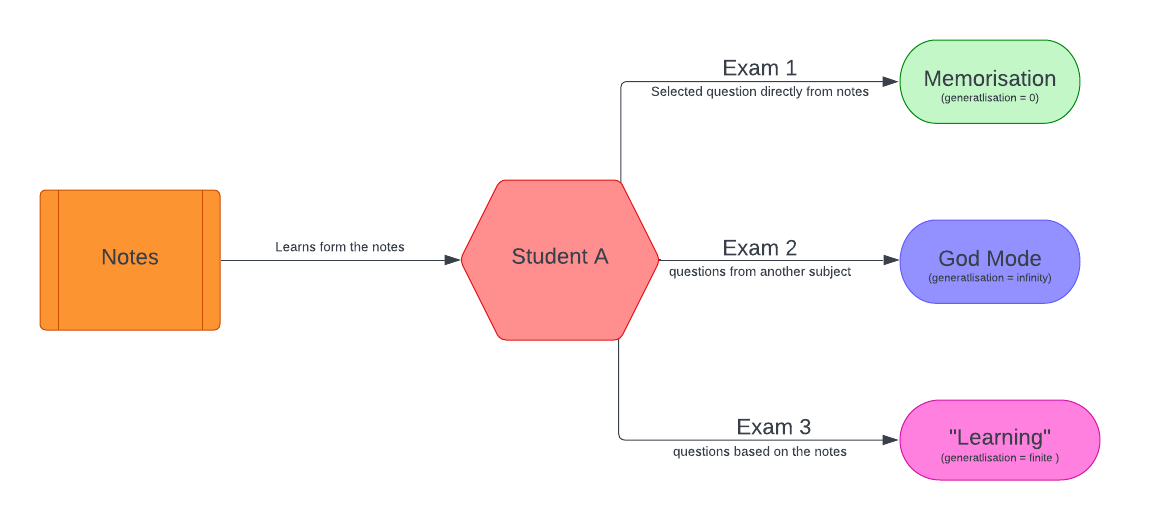
\includegraphics[width=0.85\textwidth]{figures/Generelisation.png}
    \caption{Flow chart summarizing the previous example.}
    \label{fig:Generalisation}
\end{figure}
\end{frame}

\section{Generalization}
\begin{frame}{Generalization}
\alert{Generalization} is the process of \alert{S} learning from the notes and then doing well on an exam with questions based on the notes.
\bigskip
\begin{itemize}
    \item If \alert{S} does well on an exam with questions based on the notes but not directly from them we say that the knowledge or the method of learning of \alert{S} has \alert{generalised well}. 
\end{itemize}
\end{frame}
\begin{frame}{Why is generalisation important?}
To see why generalisation is important we take two examples. One natural example from our life and one example from machine learning. 
\begin{enumerate}
    \item Consider a dog. While playing it hits a cactus tree and got hurt. So next time when it gets near a tree with needles it would be extra careful so as not to hurt itself. This would be an example of his knowledge generalising well. If for example the dog thinks that only that cactus tree can hurt it, it would keep getting hurt by other trees with needles. This is an example where the knowledge did not generalise well. 
    \item Suppose we have an algorithm for detecting whether an email is spam. We give the algorithm a bunch of emails classified as spam or not spam. Given a new email if the algorithm classifies it as spam or not spam based on the words or phrases present in the seen emails, and it produces correct results, we would say the algorithm generalised well. However given a new email if the algorithm just checks if the new email is exactly the same as the old spam email we would say the algorithm did not generalise at all.
\end{enumerate}
\end{frame}

\begin{frame}{Degrees of Generalisation}
We would like to have some way of quantifying how generalised is a learning algorithm. Consider the example at the beginning of this part,
\begin{itemize}
    \item the generalization of the learning method for doing well on the first exam is \alert{zero}. \alert{S} can just memorise everything. The generalization of memorisation is \alert{zero}.
    \item the generalization of learning method for doing well on the second exam is \alert{infinity}. \alert{S} learned from the notes for \alert{S1} but could answer questions from \alert{S2}. The generalization of this god-mode of learning is \alert{infinity}.
    \item the generalization of learning method for doing well on the third exam depends on the performance of \alert{S}. The generalization is definitely between zero and infinity and is directly proportional to how well \alert{S} did on the exam.
\end{itemize}
\end{frame}

\begin{frame}[allowframebreaks]{Overfitting vs Underfitting}
Let us take the example of a machine learning algorithm which predicts the price of a house based on its area.
    \begin{figure}
    \centering
    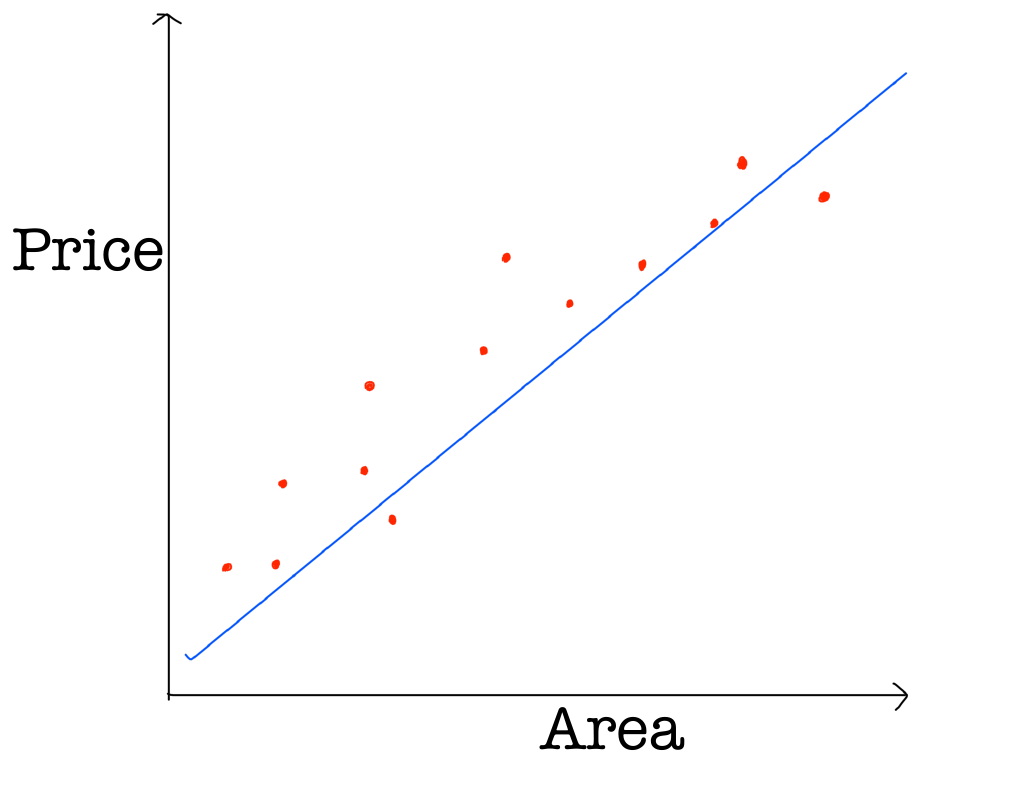
\includegraphics[width=0.4\textwidth]{figures/fitting_1.png}
    \caption{This is an example of underfitting. Very few data points are near or on the fitted line. The learning method which led to this result is similar to god-mode or the lucky escape method which helped student S do well in the second exam.}
    \label{fig:underfit}
    \end{figure}

    \begin{figure}
    \centering
    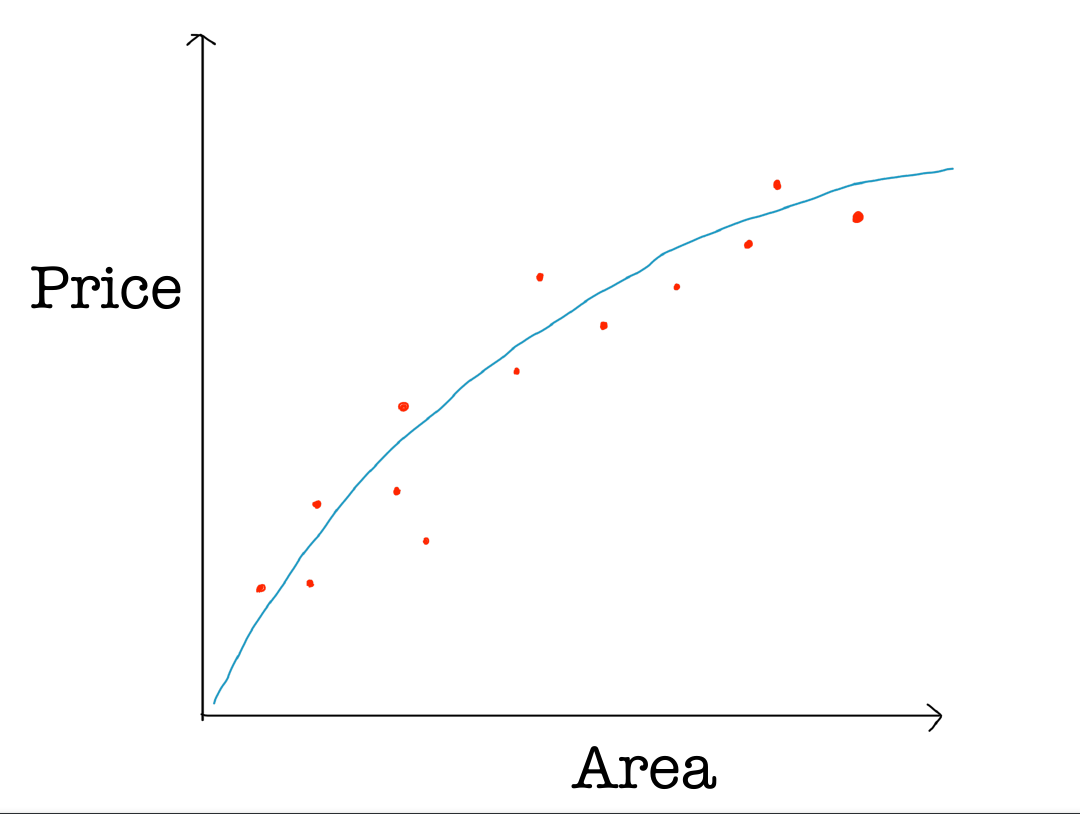
\includegraphics[width=0.5\textwidth]{figures/fitting_2.png}
    \caption{This is a good fit. The learning method which led to this result generalised well.}
    \end{figure}
    
    \begin{figure}
    \centering
    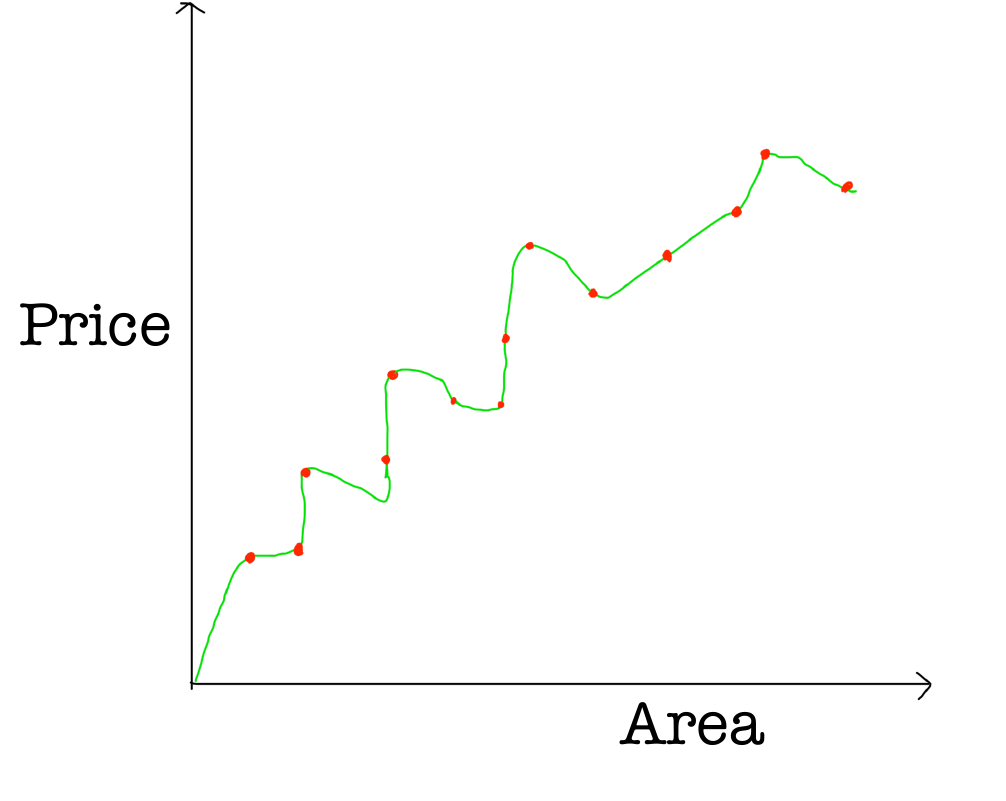
\includegraphics[width=0.5\textwidth]{figures/fitting_3.png}
    \caption{This is an example of overfitting. This situation is equivalent to memorisation. The learning method did not generalise at all. While the algorithm exactly predicts the price given any area it has already seen it would fail to make good predictions given new values of area.}
    \label{fig:overfit}
    \end{figure}
     
\end{frame}

\begin{frame}{Bias-Variance Trade-off}

As seen in the previous example doing both too well and too bad on fitting the data points resulted in undesirable outcomes. To quantify a model's fitting capacity we need to understand the concept of bias and variance.
\begin{itemize}
    \item \alert{Bias} of a model is proportional to the difference in the value of a quantity as predicted by it and the actual value of the quantity. A model has high bias if the values predicted by it are way off actual values. Whereas it has low bias if the values predicted by it are close to the actual values.
    \item \alert{Variance} of a model is the measure of the spread of the predicted values. A model with high variance has a very complicated fit to the data. A model with low variance has a simple fit to the data. 
\end{itemize}
\end{frame}

\begin{frame}{Bias-Variance Trade-off}
\begin{figure}
    \centering
    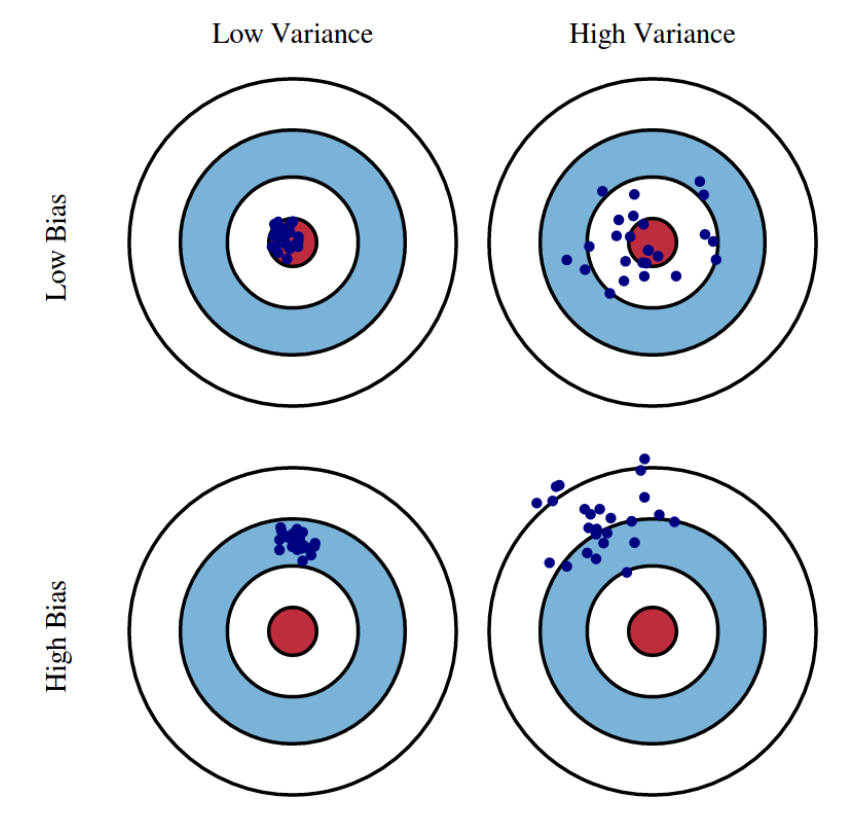
\includegraphics[width=0.4\textwidth]{figures/tradeoff.png}
    \caption{The bias-variance trade-off is of fundamental importance to machine learning. The ideal model will have low bias and low variance. A high variance model with low bias predicts value closer to the actual value but the spread of the predicted values is large. A high bias model with low variance predicts values which have a small spread but are far from the actual values. A high variance, high bias model is the worst, it predicts values with large spread which are far from the actual values.}
    \label{fig:tradeoff}
\end{figure}
\end{frame}

\section{Inductive Learning}
\begin{frame}{Inductive Learning}
Consider the teacher T, student S and subject S1 example again. The example can be summarised in the following flow-chart. 
\begin{figure}
    \centering
    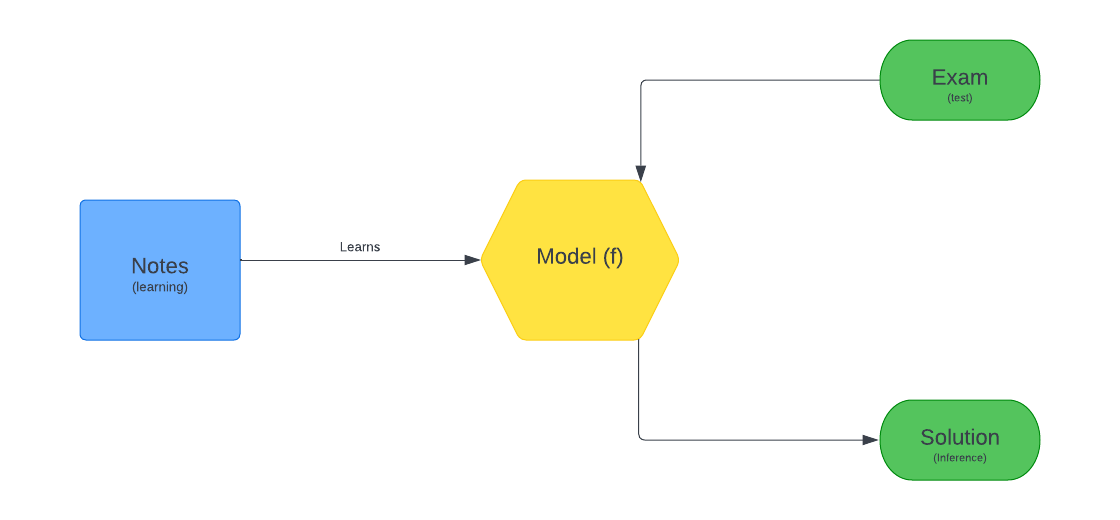
\includegraphics[width=0.85\textwidth]{figures/Model1_1.png}
    \caption{S uses the notes to learn. An exam is given to S to test its learning. S provides a solution to the exam based on his learning.}
    \label{fig:induce_example}
\end{figure}
\end{frame}

\begin{frame}{Inductive Learning}
Inductive learning refer to the general learning algorithm described by the following flow-chart. 
\begin{figure}
    \centering
    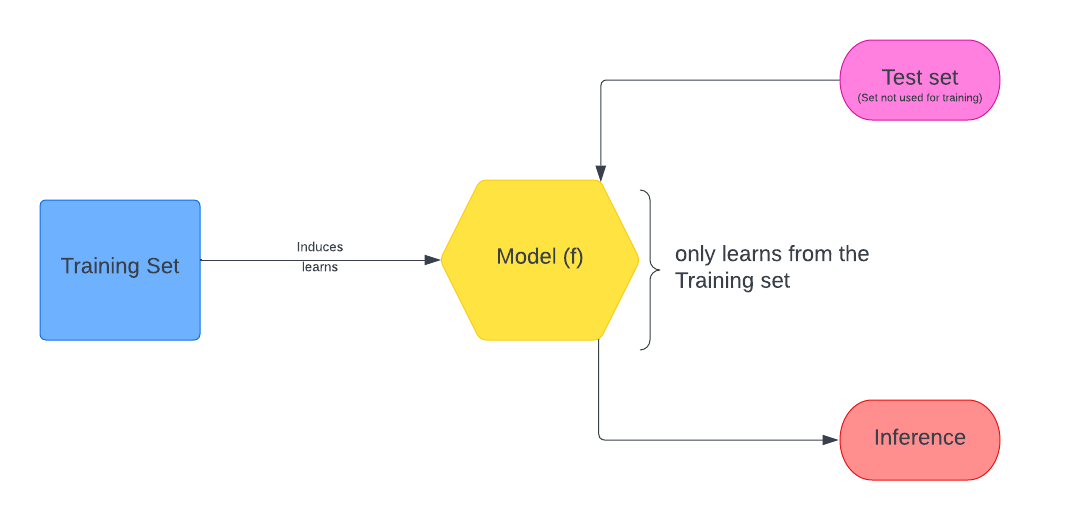
\includegraphics[width=0.75\textwidth]{figures/Model1_2.png}
    \caption{We give a set of examples as input called the \alert{\textbf{training set}}. The model learns or \alert{\textbf{induces}} from the training set and come up with a function f called the \alert{\textbf{hypothesis}}. Then we test the model's performance on a few examples which we call the \alert{\textbf{test set}}. Given an example from the test set the model using the hypothesis it induced from the training set produces an \alert{\textbf{inference}}.}
    \label{fig:gen_induction}
\end{figure}
\end{frame}

\begin{frame}{Examples}
\begin{itemize}
    \item Consider the housing price prediction example. The training set constitutes of actual prices of houses with their area. The algorithm will then come up with a line through these known data points. The equation of this line is the hypothesis of the model. We can then test the working of the model by feeding in some points that were not in the training set. Note that if we test the model on the points in the training set it may appear to perform well on the test set but fail on newer examples (the model may have overfit).
    \item In the spam detection example. The training set constitutes of emails and tagged as spam or not spam. The model will then form a hypothesis based on the training examples. The hypothesis here can be complicated it may classify an email as spam based on the words the sender and the phrases used. Once the algorithm has induced the hypothesis from the training set we can use some examples of known spam and not-spam emails not in the training set to test the hypothesis.
\end{itemize}
\end{frame}

\makepart{Structured Data and When to Use Machine Learning?}

\section{Structured and Unstructured Data}

\begin{frame}{Structured and Unstructured Data}
    \begin{itemize}
        \item Any information about a problem is data. Data on which we can ask statistical queries is called structured data. Examples of statistical queries is average, standard deviation, minimum value, maximum value, range etc.
        \item We have very good algorithms for statistical queries on structured data. For example, NumPy is a python library containing many efficient functions for statistical queries.
        \item But most of the data that we have is unstructured. We usually have data in the form of pictures or texts or audio files. These are all unstructured data. 
        \item The general structure for structured data is a table or matrix. But this also depends on the problem in hand. For example, we want to do digit classification and we are given an image as a matrix, this matrix would be unstructured data, because we cannot ask statistical queries of interest on this data.
        \item Given unstructured data converting it to structured data is very difficult. We use machine learning for this task.
    \end{itemize}
\end{frame}

\begin{frame}{The Goal of Machine Learning}
    The goal of machine learning algorithms is:
    \begin{itemize}
        \item To make unstructured data structured.
        \item \alert{Tidy} the structured data.
    \end{itemize}
\bigskip
A structured data is called \alert{tidy} if it satisfies the following three criteria:
\begin{enumerate}
    \item Every row represents one information.
    \item Every column represents one unique value.
    \item Every cell has only one value. 
\end{enumerate}
\end{frame}

\begin{frame}{Example}
Suppose we are given several X-ray images and we want to tell whether the bones are broken or not. Lets say we have a few X-ray images for which we know the percent of damage and doctor's decision of whether the bones are broken.
\bigskip
\begin{table}[]
    \centering
    \begin{tabular}{c|c|c}
    \toprule
    Picture \# & Damage Percentage & Doctor's Note\\
    \midrule
    1 & 25 & Not Broken\\
    2 & 65 & Not Broken\\
    3 & 75 & Broken\\
    \bottomrule
\end{tabular}
    \caption{Training set for our machine learning model.}
    \label{tab:training}
\end{table}
Once our model is trained on this training set, it would be able to convert X-ray images (which is unstructured data) given to it to a table similar to table 1 (which is tidy structured data).
\end{frame}

\section{When to use Machine Learning?}
\begin{frame}[allowframebreaks]{When to use Machine Learning (ML)?}
\bigskip
Following is a checklist for using machine learning to solve a problem. If any of these is not fulfilled for the problem in hand, then applying machine learning is not advisable.
\bigskip
\begin{itemize}
    \item The problem does not have an efficient analytical solution from domain knowledge. 
    \bigskip
    \begin{itemize}
        \item If an efficient analytical solution exists, using ML to solve the problem is a waste of time. At best, the ML algorithm will rediscover the already-known analytical solution. For example, using machine learning to find roots of a quadratic equation is not a good idea because we already have a formula for that. 
        \item However if the analytical solution available is not very efficient then ML algorithms can help. For example, determining the mechanism of an organic chemistry reaction has analytical solutions but these solutions require a lot of computation and generally very expensive to perform. In this case an ML algorithm can really help.
    \end{itemize}
    \bigskip
    \bigskip
    \bigskip
    \bigskip
    \item The problem does not have any analytical solution from domain knowledge or the domain knowledge is scarce.
    \bigskip
    \begin{itemize}
        \item If this is the case our only option to solve the problem is to use machine learning. For example, if we want to find the roots of polynomial of degree 5. It is mathematically proven that for such polynomials an analytical solution is not possible. But there are machine learning algorithms which can predict roots of such polynomials given their coefficients.
        \item In such cases we must make sure that we have enough data. Successful applications of machine learning usually requires a lot of data for the model to train on. We should use ML if we have a good amount of data or we can simulate a good amount of data for the problem. For example, in particle physics a lot of data is generated in big experiments such as LHC at the CERN, due to availability of huge data many machine learning algorithms are successfully deployed for particle physics experiments for classifying different particles, on the other hand in materials science the amount of data that we have is low and even simulating new data is very difficult because of which machine learning algorithms are still not very useful for materials science applications.
    \end{itemize}
\end{itemize}
\end{frame}

\begin{frame}{ML Algorithms}{}
We use machine learning  to solve mainly four types of problems, i.e regression, classification (multi or binary), and ranking. The problems mentioned above are solved using ML algorithms where our model learns from labeled or unlabeled training data, and the desired output may or may not be known.

\begin{itemize}
\item \alert{Regression:} A regression algorithm is used to predict a continuous numeric value. It is used to model the relationship between a dependent variable (also known as the target or output variable) and one or more independent variables (also known as the predictor or input variables). For example, a model might be trained to predict the price of a house based on its size, location, and other features. Linear regression and polynomial regression are common algorithms used for regression tasks.
\begin{figure}
    \centering
    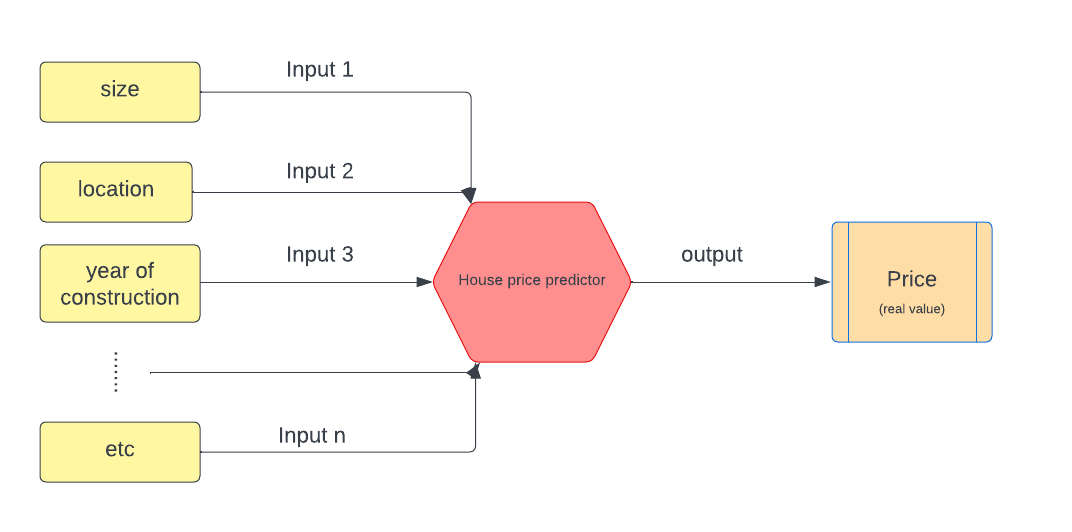
\includegraphics[width=0.5\textwidth]{figures/regression.png}
    \caption{Model for housing price predictor.}
    \label{fig:regression}
\end{figure}
\end{itemize}
\end{frame}

\section{Machine Learning (ML) Algorithms}

\begin{frame}{ML Algorithms}
\begin{itemize}
\item \alert{Binary classification:} A Binary classification algorithm is used to classify items into one of two classes. It aims to learn from labeled data and make predictions about new, unseen data. Overall, a binary classification algorithm is used to predict one of two possible outcomes by learning from labeled data and making predictions on new unseen data. For example, a model might be trained to predict whether a customer will default on a loan or not. Logistic regression, k-nearest neighbors, and decision trees are common algorithms used for classification tasks.
\begin{figure}
    \centering
    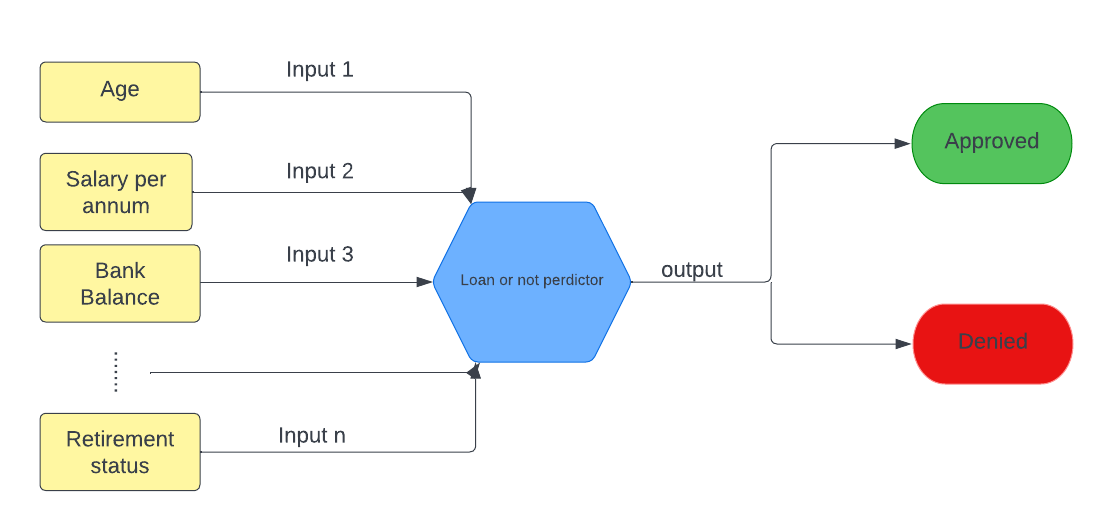
\includegraphics[width=0.5\textwidth]{figures/bi-classification.png}
    \caption{Model to predict if a  borrower will default or not.}
    \label{fig:binary classification}
\end{figure}

\end{itemize}
\end{frame}

\begin{frame}{ML Algorithms}
\begin{itemize}
\item \alert{Multi class classification:}A multi-class classification algorithm is used to classify items into one of multiple classes or categories. The goal of a multi-class classification algorithm is to learn from labeled data and make predictions about new, unseen data. Overall, a multi-class classification algorithm is used to predict one of the multiple possible outcomes, by learning from labeled data and making predictions on new unseen data. For example, a model might be trained to predict the type of fruit in an image from a set of several different fruit types.
\begin{figure}
    \centering
    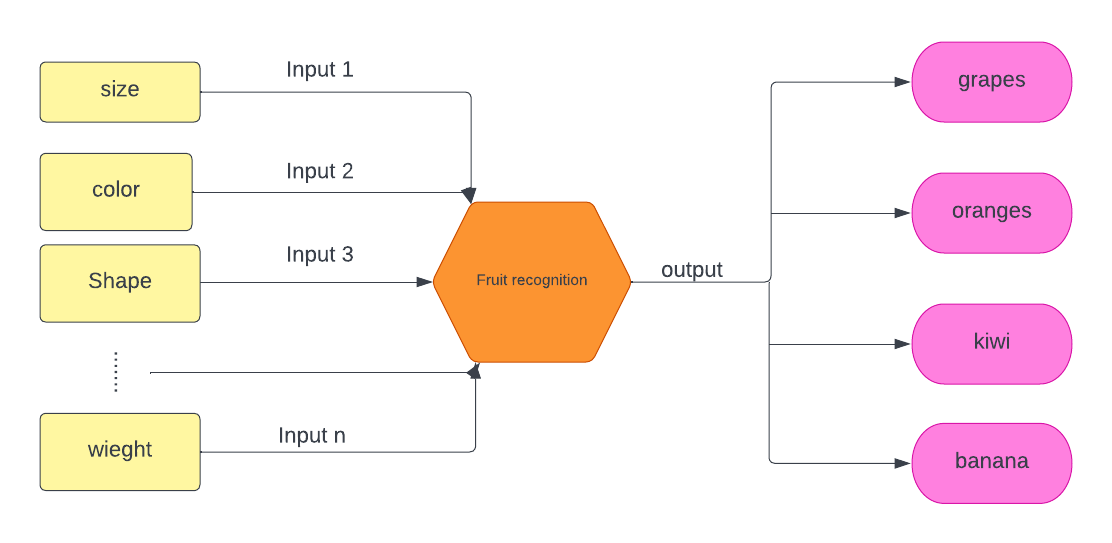
\includegraphics[width=0.5\textwidth]{figures/fruit predictor.png}
    \caption{A model of fruit predictor using ML.}
    \label{fig:multiclass classification}
\end{figure}

\end{itemize}
\end{frame}


\begin{frame}{ML Algorithms}
\begin{itemize}
\item \alert{Ranking:}A ranking algorithm is a type of machine learning algorithm that is used to predict the order of items. The goal of a ranking algorithm is to learn from labeled data and make predictions about the relative order of new, unseen items. For example, a model might be trained to predict which articles are most likely to be read by a user, or which products are most likely to be purchased by a customer.
\begin{figure}
    \centering
    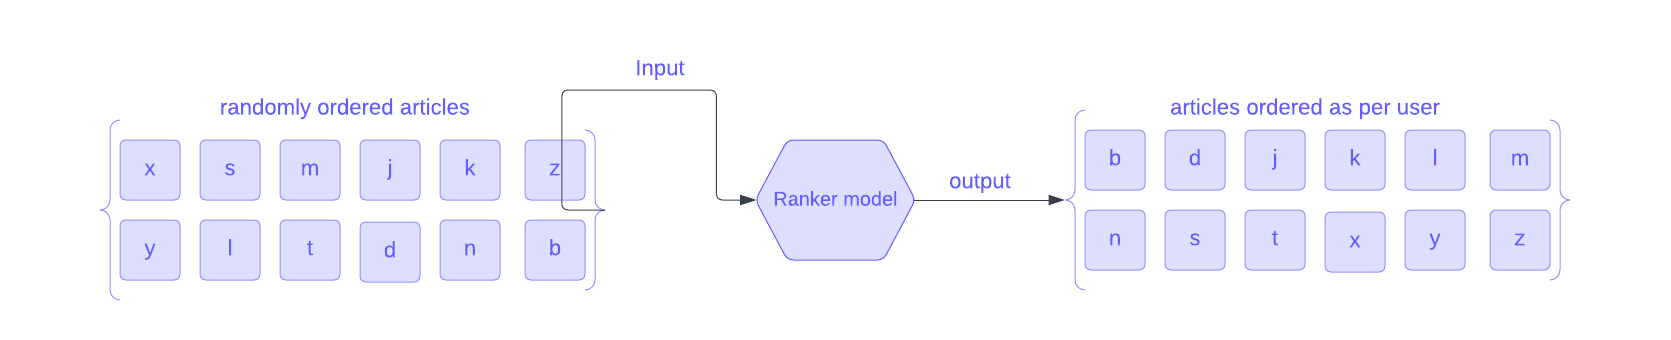
\includegraphics[width=0.9\textwidth]{figures/ranker.png}
    \caption{A model that recommends articles in order of what the reader would like the most.}
    \label{fig:multiclass classification}
\end{figure}
\end{itemize}
\end{frame}

\begin{frame}[allowframebreaks]{References}
    \begin{enumerate}
        \item CS460 (Machine Learning) 2023 lectures, Subhankar Mishra.
        \item CS460/C660 (Machine Learning) 2021, youtube playlist.
        \item Deterministic algorithm, Wikipedia.
        \item Artificial Intelligence, Wikipedia.
        \item CS4780/CS5780 (Machine Learning for Intelligent Systems), Cornell University.
        \item Introduction to Machine Learning, Coursera, Andrew Ng. 
    \end{enumerate}
\end{frame}

\end{document}